\documentclass[final,t]{beamer}

% retrieved from
% http://www-i6.informatik.rwth-aachen.de/~dreuw/latexbeamerposter.php

% {{{ preamble

% Siebel poster printer paper width -- ANSI E: 34"x44"
% Fedex Office: 24"x36" or 36"x48"

\pgfmathsetmacro{\posterheight}{34*2.54}
\pgfmathsetmacro{\posterwidth}{22*2.54}

\usepackage[orientation=landscape,size=custom,width=\posterwidth,height=\posterheight,scale=1.18]{beamerposter}

\mode<presentation>
\usetheme{uiucposter}

% {{{ additional packages

\usepackage{lipsum}
\usepackage[utf8]{inputenc}
%\usepackage{times}
\usepackage{amsmath,amsthm, amssymb, latexsym}
\usepackage[T1]{fontenc}
\usepackage{lmodern}
\usepackage{exscale}
%\usepackage[lighttt]{lmodern}
%\boldmath
\usepackage{booktabs, array}
%\usepackage{rotating} %sideways environment
\usepackage[english]{babel}
\usepackage{wrapfig}
\usepackage[skins,listings]{tcolorbox}
\usepackage{graphicx}
\graphicspath{ {./media/} }
\pgfdeclarelayer{foreground}
\pgfsetlayers{main,foreground}

% }}}

% {{{ tikz

\usepackage{tikz}
\usetikzlibrary{calc}
\usetikzlibrary{positioning}
\usetikzlibrary{fadings}
\usetikzlibrary{chains}
\usetikzlibrary{scopes}
\usetikzlibrary{shadows}
\usetikzlibrary{arrows}
\usetikzlibrary{snakes}
\usetikzlibrary{shapes.misc}
\usetikzlibrary{shapes.symbols}
\usetikzlibrary{shapes.multipart}
\usetikzlibrary{fit}
\usetikzlibrary{shapes.arrows}
\usetikzlibrary{shapes.geometric}
\usetikzlibrary{shapes.callouts}
\usetikzlibrary{decorations.text}

% }}}

% {{{ box config

\tcbset{toplevelbox/.style={%
    enhanced,
    fuzzy shadow={5mm}{-5mm}{0mm}{1mm}{black},
    colback=white,
    fonttitle=\bfseries,
    coltitle=white,
    colframe=uiucblue,
    boxsep=20pt,
    arc=10pt,
    top=0pt,
    boxrule=0pt,
    toptitle=-10pt,
    bottomtitle=-10pt,
    enlarge bottom by=1.25cm,
    titlerule=0pt,
  }
}

% }}}

% {{{ listing config

\tcbset{listing engine=listings}
\tcbset{listingbox/.style={%
    enhanced,
    %boxsep=-9pt,
    %left=15pt,
    arc=7pt,
    enlarge top by=4mm,
    %enlarge bottom by=1mm,
    boxrule=2pt,
  }
}

\definecolor{green}{RGB}{0, 180, 0}

\lstdefinestyle{custompython}{%
  %belowcaptionskip=1\baselineskip,
  breaklines=true,
  frame=none,
  xleftmargin=\parindent,
  language=Python,
  showstringspaces=false,
  basicstyle=\ttfamily,
  keywordstyle=\bfseries\color{uiucblue},
  commentstyle=\itshape\color{purple},
  identifierstyle=\color{black},
  stringstyle=\color{uiuclightblue},
  keywords=[2]{as,True,False},
  keywordstyle=[2]\bfseries\color{green!40!black},
  otherkeywords={>>>,...},
  keywordstyle=[3]\bfseries\color{blue},
  numbers=none,
  columns=flexible,
  rangebeginprefix=\>\>\>\ \#\ ,
  rangeendprefix=\>\>\>\ \#\ ,
  includerangemarker=false,
}

\newtcbinputlisting{\mylisting}[2][]{%
  listing file={#2},
  listingbox,
  listing only,
  listing options={style=custompython,linerange=#1},
}

% }}}

% Display a grid to help align images
%\beamertemplategridbackground[1cm]

% }}}


% {{{ front matter

\title{Poster Template}
\author{Poster Author \texttt{<author@illinois.edu>}}
\institute{%
  Computer Science
  $\cdot$ University of Illinois
}
\date{December 12, 2018}

% }}}

\begin{document}
\begin{frame}[fragile]{}
  \begin{columns}[t]

    % {{{ left column

    \begin{column}{.45\linewidth}
      \begin{tcolorbox}[toplevelbox,adjusted title={Problem Statement}]
        \ Fast multipole method(FMM) is a well known algorithm for N-body simulation. Naïve algorithm would have a complexity of O(N\textsuperscript{2}) because the influence of all other particles have to be calculated for each target particle. FMM reduces the complexity to O(N).However, the efficiency also highly depends on the implementation. 
        \\  Professor Andreas Kloeckner wrote a module called Boxtree for the FMM, which has high-performance parallel GPU implementation to sort all the particles into boxes, which is the first stage of the algorithm. There are also template functions for the rest of the stages, but those functions only has a baseline serial execution path, which would not exploit multicore architecture. A better implementation for is needed to replace the baseline solution.
        
      \end{tcolorbox}

      \begin{tcolorbox}[toplevelbox,adjusted title=Approach]
        \ A task graph integrating Boxtree with a runtime system is proposed as the 
          solution. The task graph is a list of funtions, which are called task. The runtime system can schdule the tasks on different processors so that different tasks can be run simultaneously with dependency specified. The runtime system
          used is called charm4py. charm4py is a high-level parallel and distributed programming framework. It's used for communication between tasks on different
          processors and specifying the execution order. With this integration, it will be able to utilize the multicore structure.
      \end{tcolorbox}

      \begin{tcolorbox}[toplevelbox,adjusted title=Tech Detail 1]
        \ The algorithm groups particles into boxes. If a box has more than the specified
        number of particles, it is further divided into four child boxes. The algorithm first calcualte the multiple expansion for all child-less boxes. It use these
        multipole expansion to calcualte the multipole expansion for higher level boxes.
        Interaction between adjacent boxes are directly calcualted, interaction between
        non-adjacent boxes can be calculated by using those multipole expansions to calculate local expansions.
        \\ First step was to identify the independent steps in the algorithm. It was clear that calculating the direct interaction is not dependent on any other stages other than the sorting stage. All the other stages depends on The second stage, which is to calculate the multipole expansion of all boxes. Stage 2 must starts at beginning. Stage 5 is evaluating multipole expansion for some boxes, which is also independent. Step 4,6 are for calculating the local expansions, which can be separated. Stage 7 is using the result of step 4,6 to calculate the local expansion for smaller boxes. Charm4py has a reduction feature which can
        collect output through different processes and process only after receives all
        the dependencies. 7 must be executed after 4 and 6 finishes. Finally, the sum up stage can run after collecting output from all other tasks.
      \end{tcolorbox}

    \end{column}

    % }}}

    % {{{ right column

    \begin{column}{.45\linewidth}
      \begin{tcolorbox}[toplevelbox,adjusted title=Tech Detail 2]
        \ Further optimization are conducted in order to achieve better performance. Not all the stages have same runtime. After measurement, it was first identified that 
        calculating direct interaction is taking significantly longer than any other stages. Thus the first approach was to break it down into smaller tasks. The optimization was to distribute the boxes onto processors evenly. Timing this section shows that some processors takes much less time to complete because the distribution of particles are not even. Thus each processor would process a similar number of particles. This is a preliminary optimization. Similar approach will be applied to other stages if possible.
      \end{tcolorbox}

      \begin{tcolorbox}[toplevelbox,adjusted title=Results]
        \  The testing was run on a analytical routines for a Green's function that is
        constant 1 everywhere. This is a sample application provided in the module. It will get each particle a particle count. The task graph is general enough to suppport many application. However,due to time constraint, this is the only one tested. Chart1 is the performance.Each task graph was run for ten times on each different data sizes. Min, median and 90 percentile are shown
        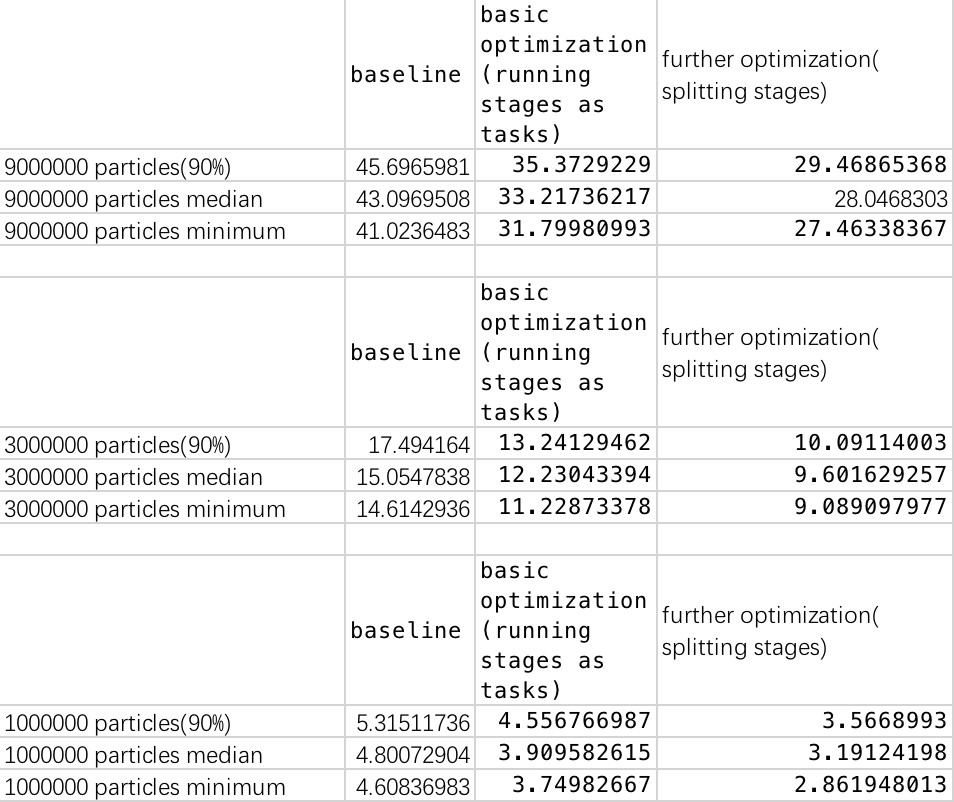
\includegraphics{chart}
      \end{tcolorbox}

      \begin{tcolorbox}[toplevelbox,adjusted title=References]
        \lipsum[8]
      \end{tcolorbox}

    \end{column}

    % }}}

  \end{columns}
\end{frame}

\end{document}

% vim: foldmethod=marker
